\section{Implementaci�n}

\begin{frame}
\begin{center}
\Huge IMPLEMENTACI�N DE LAS ARQUITECTURAS
\end{center}
\end{frame}

\subsection{Arquitecturas radix}

\begin{frame}{Radix-2 Iterativa}
  \begin{columns}[T]
    \uncover<1->{
    \begin{column}{.5\textwidth}
      \begin{center}
	    \advance\leftskip-0.2cm
	    \includegraphics[scale=0.28]{./figures/r2_8_diag.png}
      \end{center}
    \end{column}
    }
    
    \uncover<2->{
    \begin{column}{.5\textwidth}
      \begin{center}
	    \advance\leftskip-0.2cm
	    \includegraphics[scale=0.23]{./figures/radix2blocks.png}
      \end{center}
    \end{column}
    }
  \end{columns}
  
%   \begin{itemize}
%     \item<3-> Memoria
%     \item<4-> Butterfly (sumador/restador + escalamiento)
%     \item<5-> Producto por los \textit{twiddle factors}
%     \item<6-> Datapath 
%     \item<7-> Unidad de control
%   \end{itemize}  
    
\end{frame}

\begin{frame}{Radix-4 Iterativa}

%   \only<1-1>{
%    \vfill
%     \begin{center}
%       \advance\leftskip-0.2cm
%       \includegraphics[scale=0.43]{./figures/r4_16.png}
%     \end{center}
%     \vfill
%   }
  
  \begin{columns}[T]
    \uncover<1->{
    \begin{column}{.5\textwidth}
      \begin{center}
	    \advance\leftskip-0.2cm
	    \includegraphics[scale=0.3]{./figures/r4_16.png}
      \end{center}
    \end{column}
    }
    
    \uncover<2->{
    \begin{column}{.5\textwidth}
      \begin{center}
	    \advance\leftskip-0.2cm
	    \includegraphics[scale=0.23]{./figures/radix4blocks.png}
      \end{center}
    \end{column}
    }
  \end{columns}
  
%   \begin{itemize}
%     \item<3-> Memoria
%     \item<4-> Butterfly (sumador/restador + escalamiento)
%     \item<5-> Producto por los \textit{twiddle factors}
%     \item<6-> Datapath 
%     \item<7-> Unidad de control
%   \end{itemize}  
    
\end{frame}
  
\begin{frame}
   
   \begin{columns}[T]
    \uncover<1->{
    \begin{column}{.5\textwidth}
      \begin{center}
	    \advance\leftskip-0.2cm
	    \includegraphics[scale=0.275]{./figures/datapathMem.png}
      \end{center}
    \end{column}
    }
    
    \uncover<1->{
    \begin{column}{.5\textwidth}
      \begin{center}
	    \advance\leftskip-0.2cm
	    \includegraphics[scale=0.272]{./figures/r4control.png}
      \end{center}
    \end{column}
    }
  \end{columns}
  
  \begin{columns}[T]
  \begin{column}{.2\textwidth}
  \end{column}
  \begin{column}{.6\textwidth}
  \begin{center} 
    \begin{itemize}
      \item<2-> Unidad aritm�tica (incluyendo unidad de escalamiento)
      \item<3-> Multiplicador
% 	  \only<4-5>{
% 	      \begin{itemize}
% 	        \item<4-> Algoritmo Cordic
% 	        \item<5-> Multiplicador comlejo eficiente
% 	      \end{itemize}
% 	  } 
      \item<4-> Memoria
%       \only<7-8>{
% 	      \begin{itemize}
% 	        \item<7-> Radix-2: Dual-port RAM
% 	        \item<8-> Radix-4: Triple in/Triple out RAM
% 	      \end{itemize}
% 	  }
      \item<5-> Datapath
      \item<6-> Unidad de control
    \end{itemize}
  \end{center}
  \end{column}
  \begin{column}{.2\textwidth}
  \end{column}
  \end{columns}
\end{frame}

% \subsection{Unidad aritmética}
% \begin{frame}{}
%   \begin{columns}[T]
%     \uncover<1->{
%     \begin{column}{.5\textwidth}
%       \begin{itemize}
%         \item<1-> Suma y resta entre dos puntos         
%       \end{itemize}
%       \uncover<2->{
%         \begin{center}
%         \advance\leftskip-0.2cm
%         \includegraphics[scale=0.45]{./figures/butterfly_esq.png}
%       \end{center}
%       }
%     \end{column}
%     }
%     
%     \uncover<3->{
%     \begin{column}{.5\textwidth}
%       \begin{itemize}
%         \item<3-> Operaciones entre cuatro puntos
%         \item<4-> Datapath interno          
%       \end{itemize}
%       \uncover<5->{
%         \begin{center}
%         \advance\leftskip-0.2cm
%         \includegraphics[scale=0.25]{./figures/firefly.png}
%       \end{center}
%       }
%     \end{column}
%     }
%     \end{columns}
%   
% \end{frame}
% 
% \subsection{Multiplicación}
% 
% \begin{frame}{Algoritmo Cordic}
%   \begin{itemize}
%     \item<1-> Rotaciones en base a microrotaciones
%     \item<2-> Microrotaciones sucesivas
%     \item<4-> Arquitectura desenrrollada
% %     \begin{itemize}
% %       \item<2-> Permite realizar todo el procesamiento en un solo ciclo de clock
% %       \item<3-> Permite la implementación de un \textit{pipeline} entre las etapas de rotación
% %     \end{itemize}
%     \item<5-> Preprocesador
%     \item<6-> Escalado final
%   \end{itemize}
%   
%   \begin{columns}[T]
%     \uncover<3-8>{
%       \begin{column}{.3\textwidth}
%          \begin{center}
%            \advance\leftskip-0.2cm
%            \includegraphics[scale=0.45]{./figures/cordic.png}
%          \end{center}
%       \end{column}
%     }
%     \begin{column}{.6\textwidth} 
%       \only<7-7>{
%         \begin{center}
%           \advance\leftskip-0.2cm
%           \includegraphics[scale=0.3]{./figures/cordicBlocks.png}
%         \end{center}
%       }
%       \only<8-8>{
%         \begin{center}
%           \advance\leftskip-0.2cm
%           \includegraphics[scale=0.3]{./figures/uCordicBlocks.png}
%         \end{center}
%       }
%     \end{column}
%   \end{columns}
% \end{frame}
% 
% \begin{frame}{Multiplicador complejo}
% \begin{itemize}
%   \item<1-> Memoria para los factores
%   \item<2-> Preprocesador
%   \item<3-> Multiplicación compleja
%   \uncover<4->{
%   \begin{center}
%     \advance\leftskip-0.2cm
%     \includegraphics[scale=0.3]{./figures/multBlocks.png}
%   \end{center}
%   }
% \end{itemize}
% \end{frame}
% 
% \subsection{Memoria}
% \begin{frame}{}
% 
%   \begin{columns}[T]
%     \uncover<1->{
%     \begin{column}{.5\textwidth}
%       \begin{center}
% 	    \advance\leftskip-0.2cm
% 	    \includegraphics[scale=0.3]{./figures/dportRam.png}
%       \end{center}
%       
%       \begin{itemize}
%         \item<2-> Tipo dual port RAM
%         \item<3-> Un puerto de lectura y uno de esccritura
%       \end{itemize}
%     \end{column}
%     }
%     
%     \uncover<1->{
%     \begin{column}{.5\textwidth}
%       \begin{center}
% 	    \advance\leftskip-0.2cm
% 	    \includegraphics[scale=0.23]{./figures/tripleRAM.png}
%       \end{center}
%       \begin{itemize}
%         \item<4-> En cada operación se necesitan leer tres datos y escribir tres datos
%         \item<5-> Tres puertos de lectura y tres puertos de escritura
%         \item<6-> tres sub-bloques dual port RAM
%       \end{itemize}
%       \end{column}
%      }
%     
%     \end{columns}
%   
% \end{frame}
% 
% \subsection{Datapath}
% \begin{frame}{Datapath general}
% 
%   \begin{itemize}
%     \item<1-> Hay dos tipos de operaciones posibles
%     \begin{itemize}
%       \Fontitit
%       \item<2-> Traspaso de datos en memoria
%       \item<3-> Operación aritmética entre dos datos
%     \end{itemize}
%   \end{itemize}
%   
%   \begin{columns}[T]
%     \uncover<4->{
%       \begin{column}{.5\textwidth}
%         \begin{center}
%           \advance\leftskip-0.2cm
%           \includegraphics[scale=0.27]{./figures/datapath.png}
%         \end{center}
%       \end{column}
%       }
%       \uncover<4->{
%       \begin{column}{.5\textwidth}
%         \begin{center}
%           \advance\leftskip-0.2cm
%           \includegraphics[scale=0.27]{./figures/datapathR4.png}
%         \end{center}
%       \end{column}
%       }
%   \end{columns}
%       
% \end{frame}
% 
% \begin{frame}{Datapath Radix-2}  
% 
%   \only<1-1>{
%   Etapa inicial
%   \begin{columns}[T]
%     \begin{column}{.5\textwidth}
%       \begin{center}
%         \advance\leftskip-0.2cm
%         \includegraphics[scale=0.20]{./figures/datapath_mem1.png}
%       \end{center}
%     \end{column}
%     
%     \begin{column}{.5\textwidth}
%       \begin{center}
%         \advance\leftskip-0.2cm
%         \includegraphics[scale=0.20]{./figures/datapath_but1.png}
%       \end{center}
%     \end{column}
%   \end{columns}
%   }
%   
%   \only<2-2>{
%   Etapas intermedias
%   \begin{columns}[T]
%     \begin{column}{.5\textwidth}
%       \begin{center}
%         \advance\leftskip-0.2cm
%         \includegraphics[scale=0.20]{./figures/datapath_memint.png}
%       \end{center}
%     \end{column}
%     
%     \begin{column}{.5\textwidth}
%       \begin{center}
%         \advance\leftskip-0.2cm
%         \includegraphics[scale=0.20]{./figures/datapath_butint.png}
%       \end{center}
%     \end{column}
%   \end{columns}
%   }
%   
%   \only<3-3>{
%   Etapa final
%   \begin{columns}[T]
%     \begin{column}{.5\textwidth}
%       \begin{center}
%         \advance\leftskip-0.2cm
%         \includegraphics[scale=0.20]{./figures/datapath_memf.png}
%       \end{center}
%     \end{column}
%     
%     \begin{column}{.5\textwidth}
%       \begin{center}
%         \advance\leftskip-0.2cm
%         \includegraphics[scale=0.25]{./figures/datapath_butf.png}
%       \end{center}
%     \end{column}
%   \end{columns}
%   }
%   
% \end{frame}
% 
% \begin{frame}{Datapath Radix-4}
%   \only<1-1>{
%   Etapa inicial
%   \begin{columns}[T]
%     \begin{column}{.5\textwidth}
%       \begin{center}
%         \advance\leftskip-0.2cm
%         \includegraphics[scale=0.28]{./figures/datapathR4_mem_ini.png}
%       \end{center}
%     \end{column}
%     
%     \begin{column}{.5\textwidth}
%       \begin{center}
%         \advance\leftskip-0.2cm
%         \includegraphics[scale=0.28]{./figures/datapathR4_arit_ini.png}
%       \end{center}
%     \end{column}
%   \end{columns}
%   }
%   
%   \only<2-2>{
%   Etapas intermedias
%   \begin{columns}[T]
%     \begin{column}{.5\textwidth}
%       \begin{center}
%         \advance\leftskip-0.2cm
%         \includegraphics[scale=0.28]{./figures/datapathR4_mem_int.png}
%       \end{center}
%     \end{column}
%     
%     \begin{column}{.5\textwidth}
%       \begin{center}
%         \advance\leftskip-0.2cm
%         \includegraphics[scale=0.28]{./figures/datapathR4_arit_int.png}
%       \end{center}
%     \end{column}
%   \end{columns}
%   }
%   
%   \only<3-3>{
%   Etapa final
%   \begin{columns}[T]
%     \begin{column}{.5\textwidth}
%       \begin{center}
%         \advance\leftskip-0.2cm
%         \includegraphics[scale=0.28]{./figures/datapathR4_mem_fin.png}
%       \end{center}
%     \end{column}
%     
%     \begin{column}{.5\textwidth}
%       \begin{center}
%         \advance\leftskip-0.2cm
%         \includegraphics[scale=0.28]{./figures/datapathR4_arit_fin.png}
%       \end{center}
%     \end{column}
%   \end{columns}
%   }
%   
% \end{frame}
% 
% \subsection{Escalamiento}
% 
% \begin{frame}{Unidad de escalamiento}
%   \begin{itemize}
%     \item<1-> Hay riesgo de \textit{overflow}
%     \item<2-> 1 bit por etapa
%     \item<3-> División por 2
%     \begin{itemize}
%       \item<4-> Truncamiento
%       \item<5-> Redondeo
%     \end{itemize} 
%     \item<6-> Activación dinámica y diferenciada por etapa
%   \end{itemize}
%   
%   \uncover<7->{
%   \begin{center}
%     \advance\leftskip-0.2cm
%     \includegraphics[scale=0.42]{./figures/escBlocks.png}
%   \end{center}
%   }
%   
% \end{frame}
% 
% \subsection{Unidad de Control}
% 
% \begin{frame}{Unidad de Control - Descripción}
%   \begin{itemize}
% %     \item<1-> La unidad de control debe controlar el funcionamiento de la arquitectura
% %     \begin{itemize}
% %       \item<2-> Configuración del datapath
% %       \item<3-> Control de la memoria
% %       \item<4-> Generación de los twiddle factors
% %       \item<5-> Control del escalamiento para cada etapa
% %     \end{itemize}
%     \item<1-> El control se realiza mediante dos contadores
%     \begin{itemize}
%       \item<2-> Un contador de etapas, \textit{stg\_ctr}
%       \item<3-> Un contador de puntos, \textit{ptr\_ctr}
%     \end{itemize}  
%     \item<4-> El tipo de operación se determina analizando una posición del contador de
%     puntos 
%     \uncover<5-7>{
%     \begin{columns}[T]
%       \begin{column}{.5\textwidth}
% 	    \begin{center}
% 	      \advance\leftskip-0.2cm
% 	      \includegraphics[scale=0.22]{./figures/r2conts.png}
% 	    \end{center}
% 	    \begin{columns}[T]
% 	      \begin{column}{.2\textwidth}
% 	      
% 	      \end{column}
%           \begin{column}{.8\textwidth}
% 	        \begin{itemize}
% 	          \item<6-> `0': operación en memoria
% 	          \item<6-> `1': operación aritmética
% 	        \end{itemize}
% 	      \end{column}
% 	      \begin{column}{.1\textwidth}
% 	      
% 	      \end{column}
% 	    \end{columns}
% 	  \end{column}
% 	  
% 	  \begin{column}{.5\textwidth}
% 	    \begin{center}
%           \advance\leftskip-0.2cm
%           \includegraphics[scale=0.22]{./figures/r4conts.png}
%         \end{center}
%         \begin{columns}[T]
% 	      \begin{column}{.2\textwidth}
% 	      
% 	      \end{column}
%           \begin{column}{.8\textwidth}
%           \begin{itemize}
%             \item<7-> `00': operación a memoria A
%             \item<7-> `01': operación a memoria B
%             \item<7-> `10': operación a memoria C
%             \item<7-> `11': operación aritmética
%           \end{itemize}
%           \end{column}
% 	      \begin{column}{.1\textwidth}
% 	      
% 	      \end{column}
% 	    \end{columns}
% 	  \end{column}
%     \end{columns}
%     }
%  
% %     \item<6-> La memoria se direcciona con el contador de puntos
% %     \item<7-> El ángulo correspondiente al twiddle factor se genera en base a ambos contadores
%   \end{itemize}
% \end{frame}
% 
% \begin{frame}{Unidad de Control - Máquinas de estado}
%   
%   \begin{itemize}
%     \item<1-> La unidad de control funciona en base a dos máquinas de estados
%     \begin{itemize}
%       \Fontitit
%       \item<2-> Una máquina de estados principal. Inicialización y reset.
%       \item<4-> Una máquina de estados operativa. Configuración del datapath.
%     \end{itemize}
%   \end{itemize}
%   
%   \begin{columns}[T]
%     \uncover<3-5>{
%       \begin{column}{.4\textwidth}
%         \begin{center}
%           \advance\leftskip-0.2cm
%           \includegraphics[scale=0.35]{./figures/SMr2gen.png}
%         \end{center}
%       \end{column}
%     }
%     
%     \uncover<5-5>{
%       \begin{column}{.6\textwidth}
%         \begin{center}
%           \advance\leftskip-0.2cm
%           \includegraphics[scale=0.19]{./figures/SMr2op.png}
%         \end{center}    
%       \end{column}
%     }
%   \end{columns}
% \end{frame}
% 
% \subsection{Diseño final}
% 
% \begin{frame}{Diseño final de la arquitectura radix-2}
%   \begin{center}
%     \advance\leftskip-0.2cm
%     \includegraphics[scale=0.4]{./figures/datapathMem.png}
%   \end{center}
% \end{frame}
% 
% \begin{frame}{Diseño final de la arquitectura radix-4}
%   \begin{center}
%     \advance\leftskip-0.2cm
%     \includegraphics[scale=0.4]{./figures/datapathR4control.png}
%   \end{center}
% \end{frame}
% 
% 
% \subsection{Interfaces de las arquitecturas}
% \begin{frame}{}%{Interfaces de las arquitecturas}
%   \begin{center}
%     \advance\leftskip-0.2cm
%     \includegraphics[scale=0.5]{./figures/arcInterf.png}
%   \end{center}
% \end{frame}